\documentclass[12pt]{article}
\usepackage{graphicx}
  
%
% Title[Enter title of the experiment here]
\title{EE230: Experiment No.8\\
Logarithmic Amplifier}

% Author[Enter details of author here]
\author{Mudavath vishnuvardhan,200070044}

% begin the document.
\begin{document}

% make a title page.[this creates title page]
\maketitle

%\textbf{ * All experiment reports may not contain all fields in this format,This document is just for your reference*} 

\section{Overview of the experiment} %[This segment creates Section as seen in document]

\subsection{Aim of the experiment}%[This segment creates sebsections under the same section]

We have to plot IV characteristic using the given data and then do the simulation and calculations for linear region.

\subsection{Methods}




I first plotted the IV characteristic using the given data and observed the linear region for the same.Then I calculated the saturation current( \(I_{s}\)), n,R and wrote expression for \(V{out1}\) and found \(V_{offset}\) and ratio of R3 and R2.I took random value for R1.Then I did the simulation and adjusted \(V_{offset}\) to make the \(V_{out}\) vs ln\(V_{in}\) with slope 1 amd passing through (0,0).

\section{Design}%[To add multiple sections, keep appending blocks like this]
IV characteristic:\newline
\begin{figure}

\centering
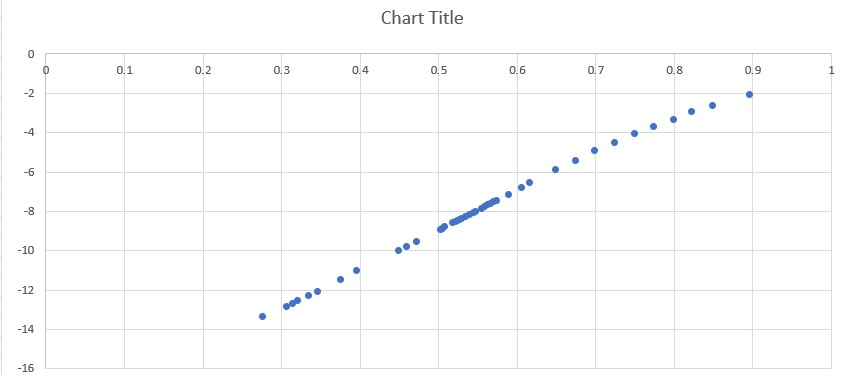
\includegraphics[scale = 0.7]{plot.jpg}
\end{figure}
\newpage
Linear region starts from V=0.397, ln(Id)=-11.0747 and end at V=0.7, ln(Id)= -4.98.\newline
For calculation of \(I_{s}\) and n:\newline
 
 \begin{equation}
     ln(I_{d})=(V_{d})/n(V_{T})+ln(I_{s})
     \end{equation} 
\begin{equation}
     (ln(I_{d})+11.0747)/(V_{d}-0.397)=(-4.98+11.0747)/(0.7-0.397)\newline
     \end{equation} 
     \begin{equation}
     ln(I_{d})=20.1145V_{d}-18.61\newline
     \end{equation} 
     \begin{equation}
     ln(I_{s})=-18.61\newline
     \end{equation} 
     \begin{equation}
     I_{s}=8.275nA\newline
     \end{equation} 
\newpage
     \begin{equation}
     1/nV_{T}=20.1145\newline
\end{equation} 
\begin{equation}
n=2
\end{equation} 
\begin{equation}
R=411ohm
 \end{equation}     
 
 \begin{equation}
     V_{out1}=-nV_{T}ln(V_{in})+nV_{T}ln((I_{s})R)\newline
\end{equation} 
\begin{equation}
     V_{out1}=-0.05ln(V_{in})-0.65\newline
\end{equation} 
\begin{equation}
     a_{1}=-0.05\newline
\end{equation}      
 \begin{equation}
     a_{2}=-0.65\newline
\end{equation} 
\begin{equation}
     V_{offset}=a_{2}/2=-0.325V\newline
\end{equation} 
\begin{equation}
1/(1+(R_{3}/R_{2}))=-a_{1}\newline
\end{equation} 
\begin{equation}
R_{3}:R_{2}=19:1
 \end{equation}     
Let \(R_{1}\)=1kohm
\newpage
\begin{figure}

\centering
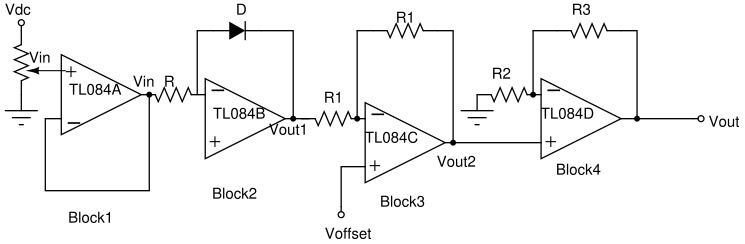
\includegraphics[scale = 0.9]{log_amp.png}
\end{figure}
 %equations are to inserted in this manner.


%\textbf{(copy-paste from handout will be counted as plagiarism).} 

%\textbf{this command prints text inside it in bold style}


\section{Simulation results}%[One more section]
\subsection{Code snippet}
logarithmic amp\\
.include TL084.txt\\
.include 1N4148\_1.txt\\

x1 1 20 3 4 2 TL084\\
vcc1 3 0 15\\
vcc2 4 0 -15\\
vin 1 0 dc 0\\
rt 20 2 0\\
x2 0 5 7 8 6 TL084\\ 
r 2 5 411\\
d1 5 6 1N4148\\
VCC3 7 0 +15\\
vcc4 8 0 -15\\
x3 10 9 12 13 11 TL084\\
r11 6 9 10K\\
r12 9 11 10k\\
vcc5 12 0 15\\
vcc6 13 0 -15\\
voff 10 0 -0.325\\
X4 11 14 15 16 17 TL084\\
r2 14 0 1k\\
r3 14 17 14.5k\\
vcc7 15 0 15\\
vcc8 16 0 -15\\
.dc vin 0.1 10 0.1\\
.control\\
run\\
plot v(17)\\ 
print v(17)\\
.endc \\
.end\\







\subsection{Simulation results}

\begin{figure}[h!]

\centering
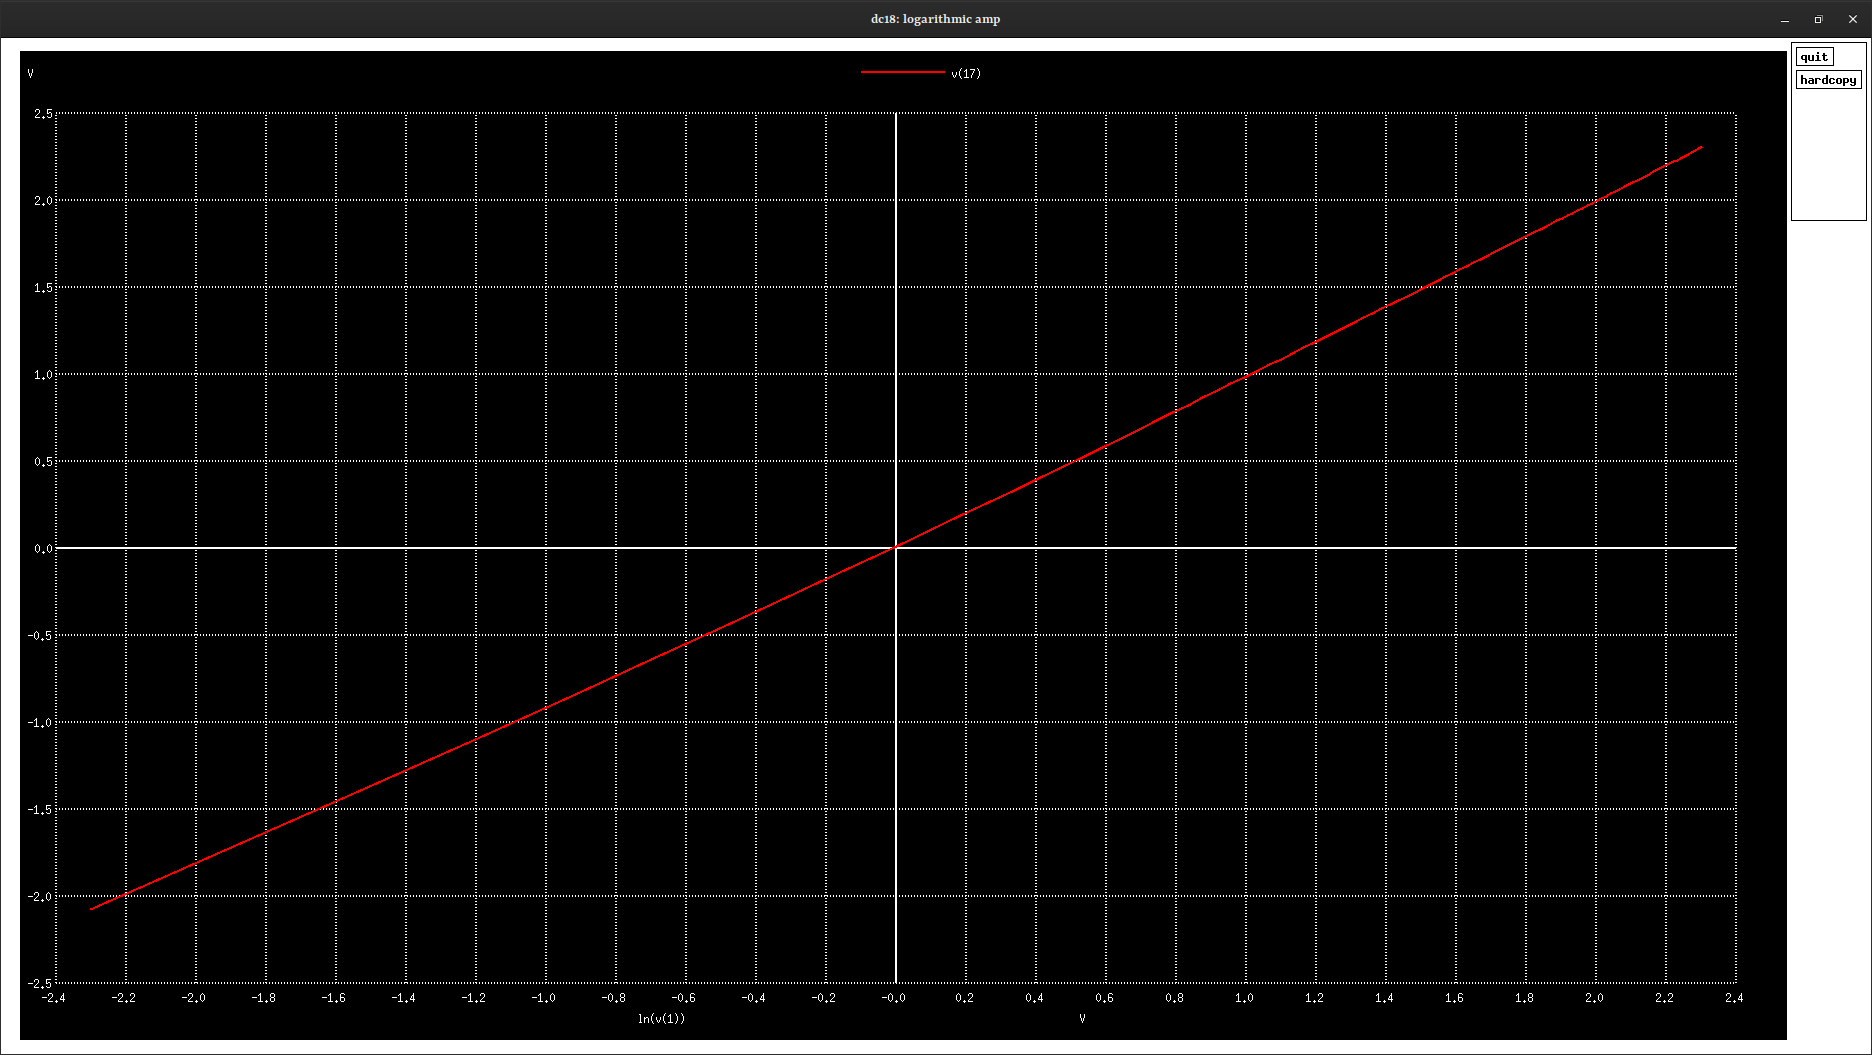
\includegraphics[scale = 0.2]{vout_ln(vin).png}
\end{figure}

\begin{figure}[h!]

\centering
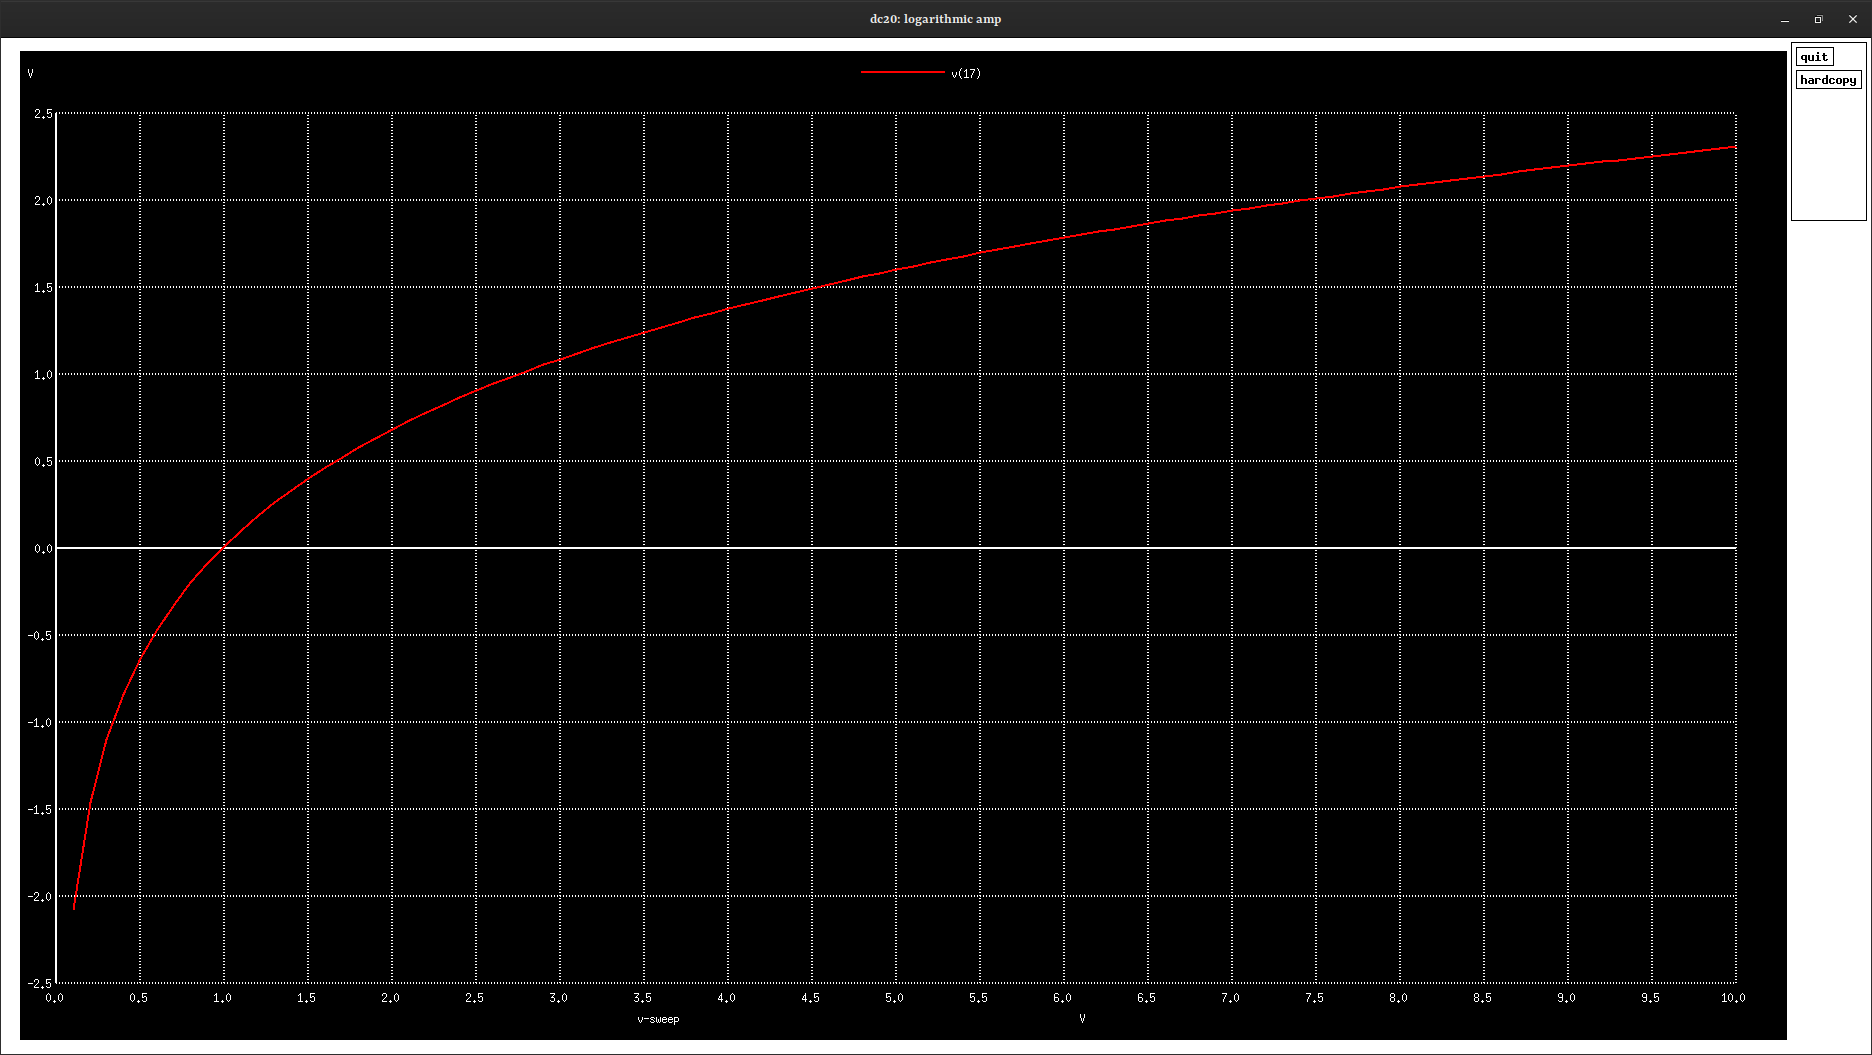
\includegraphics[scale = 0.2]{vout_vin.png}
\end{figure}
\newpage

\section{Experimental results}

I got the following results:\newline
\(I_{s}\)=8.275nA, n=2, R=411ohm, \(V_{out1}\)=-0.325V,\newline
\(R_{1}\)=1kohm, \(R_{3}\):\(R_{2}\)=19:1
\section{Experiment completion status}
I have completed all parts of the experiment in lab only.

\end{document}
